\documentclass[12pt, a4paper, titlepage]{report}

\usepackage{graphicx}   % Images
\usepackage{enumitem}   % Pretty lists
\usepackage{listings}   % Code listings

\usepackage[backend=bibtex]{biblatex}   % Bibliography
\bibliography{Maturawork2023}


\title{Maturaarbeit}
\author{Lars Hoesli}
\date{December 2023}

% Make title, author and date referencable
\makeatletter\let\inserttitle\@title\makeatother
\makeatletter\let\insertauthor\@author\makeatother
\makeatletter\let\insertdate\@date\makeatother


\begin{document}

\begin{titlepage}
    \centering

	 % Title
    \Huge{\textbf{\inserttitle}}
    \par
    \LARGE{\insertauthor}

    \large{\insertdate}
    \vspace{2cm}

    % Title picture
    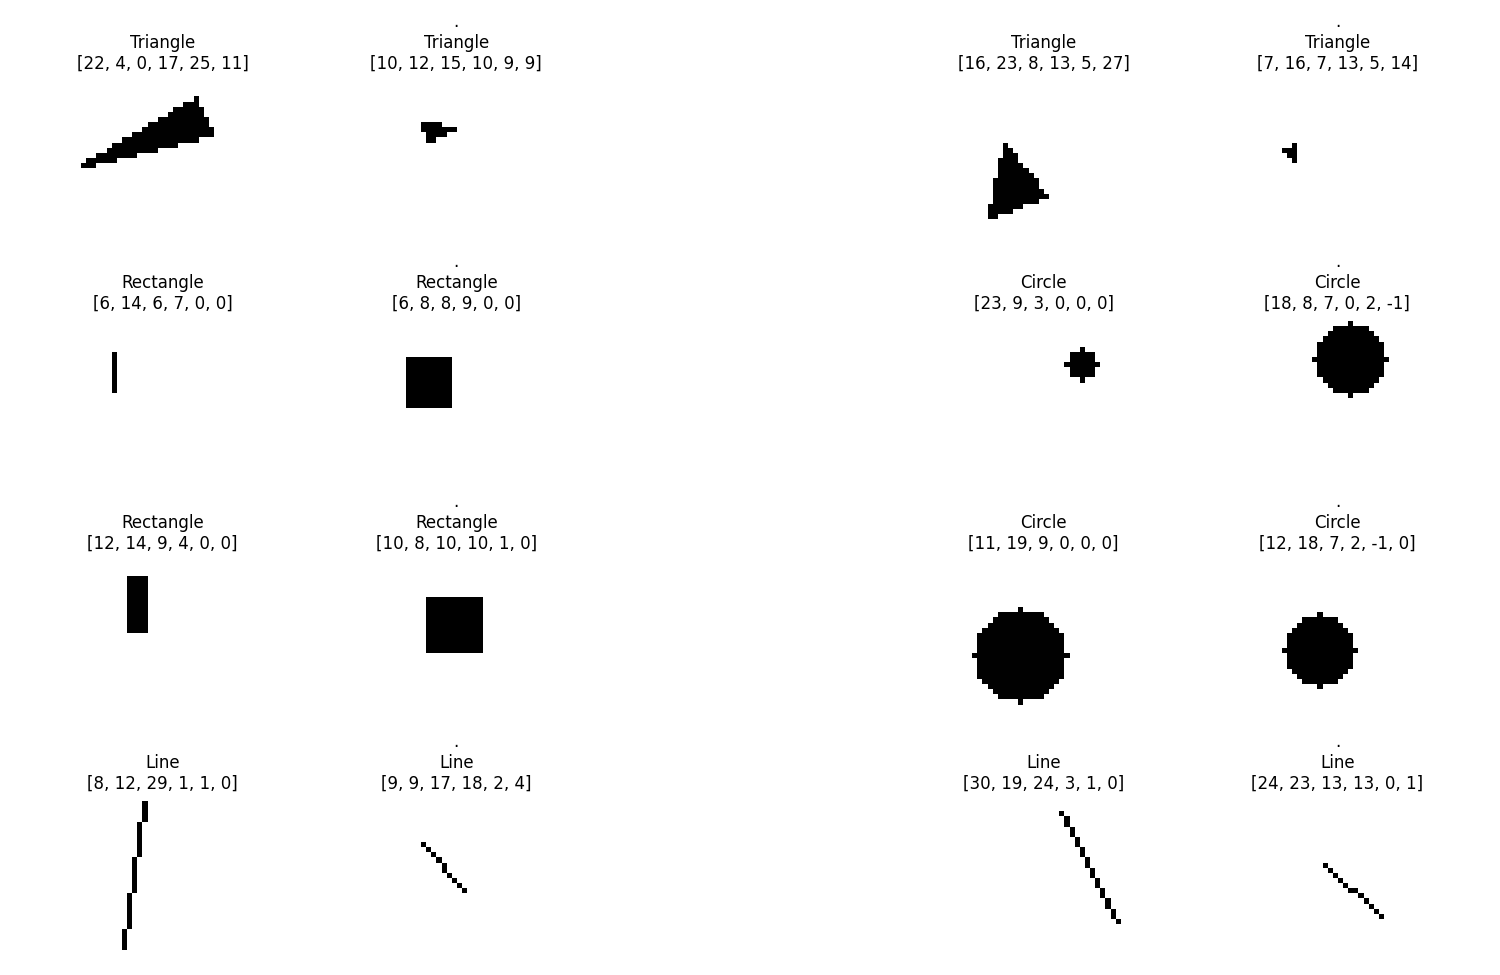
\includegraphics[width=1.0\textwidth]{../rc/images/all_shapes_approx_visual1.png}
    \vfill
    \begin{abstract}
		 This paper examines a particular approach for converting raster images containing clearly visible shapes into a vector representation.
		 It is demonstrated how a neural network can learn to extract the necessary data through training with on-the-fly generated data.
    \end{abstract}
\end{titlepage}


\tableofcontents


\chapter{Introduction}

Images have become an important part of everyday live, most of which are stored digitally, which is making the search for effective storage of images an essential, well researched aspect of computer science.
Many different formats and compression have emerged, the most influential of which can be categorized into two main categories - vector and raster formats.

\section{Vector and Raster Graphics}

Vector and raster graphics are two fundamentally different approaches on how to represent the content of an image. Both have advantages in representing a certain kind of image, and are less appropriate in other situations. While raster images store the color values of small parts of a given picture - often called pixels - to approximate what the image looks like, vector formats rather store a specification for what shapes can be seen, similar to how humans describe images.

Both methods have pros and cons, and are more appropriate for certain situations than others. But vector formats have many advantages for storing images that are easily describable in shapes, especially shapes made up of one-colored areas or easily describable gradients. In such cases, vector graphics can represent those shapes more precise, with infinite resolution, while being less storage intensive at the same time. Raster formats in turn are better suited for images without easily distinguishable shapes, such as portraits or landcape images.

While format conversions among raster or vector formats and from vector to raster graphics can be done with a multitude of programs, the conversion from a raster image to a vector representation proves to bee more challenging, especially because the shapes and their features seen in the input image have to be recognized, which is not a easily solvable problem. Many factors can make it much more difficult, such as contrasts in different strengths, noise, and gradients that make it impossible to work with fixed thresholds to detect the contoures of shapes. With different manipulations, that one can apply to a given image, edge detection is made possible. That does not solve the problem though, since the composition of those edges still is difficult to do algorithmically.
With deep learning those problems can somewhat be overcome, since the model itself can recognize the shapes, in a similar manner as humans do. Deep learning models have their own difficulties, of which accumulating training data is a big limitation.

Therefore a way to convert raster images into a vector format is beneficial, and is not yet a solved problem. This is why I have chosen to do my matura thesis on the topic of raster to vector conversion.


\pagebreak

\section{}
\subsection{Activation Functions}

\section{Architectures of Neural Networks}

Deep neural networks can be structured in different ways, leading to different kinds of traits that are beneficial in certain situations over others. For raster to vector conversion the following architectures are especially interesting.

\subsection{Convolutional Neural Networks}

A convolutional neural network (CNN) is a type of neural network that uses a convolutional layer to extract features from an input image. It is useful to reduce the information of the single pixels to a sequence of single features, that fully connected layers then can learn to connect. In order to extract the relevant features, it uses different \emph{kernels}, which are moved through the images using a certain \emph{stride} value, and applied to the pixel values. The \emph{kernel} and \emph{stride} values can be used to reduce the information for the following layers directly. Alternatively after each convolution, a certain function can be applied, which reduces the processed features. A common architecture consists of repeating convolution and pooling layers, and finally fully connected neuronal layers as it is seen in \ref{fig:cnn_architecture}.

{
	\centering
	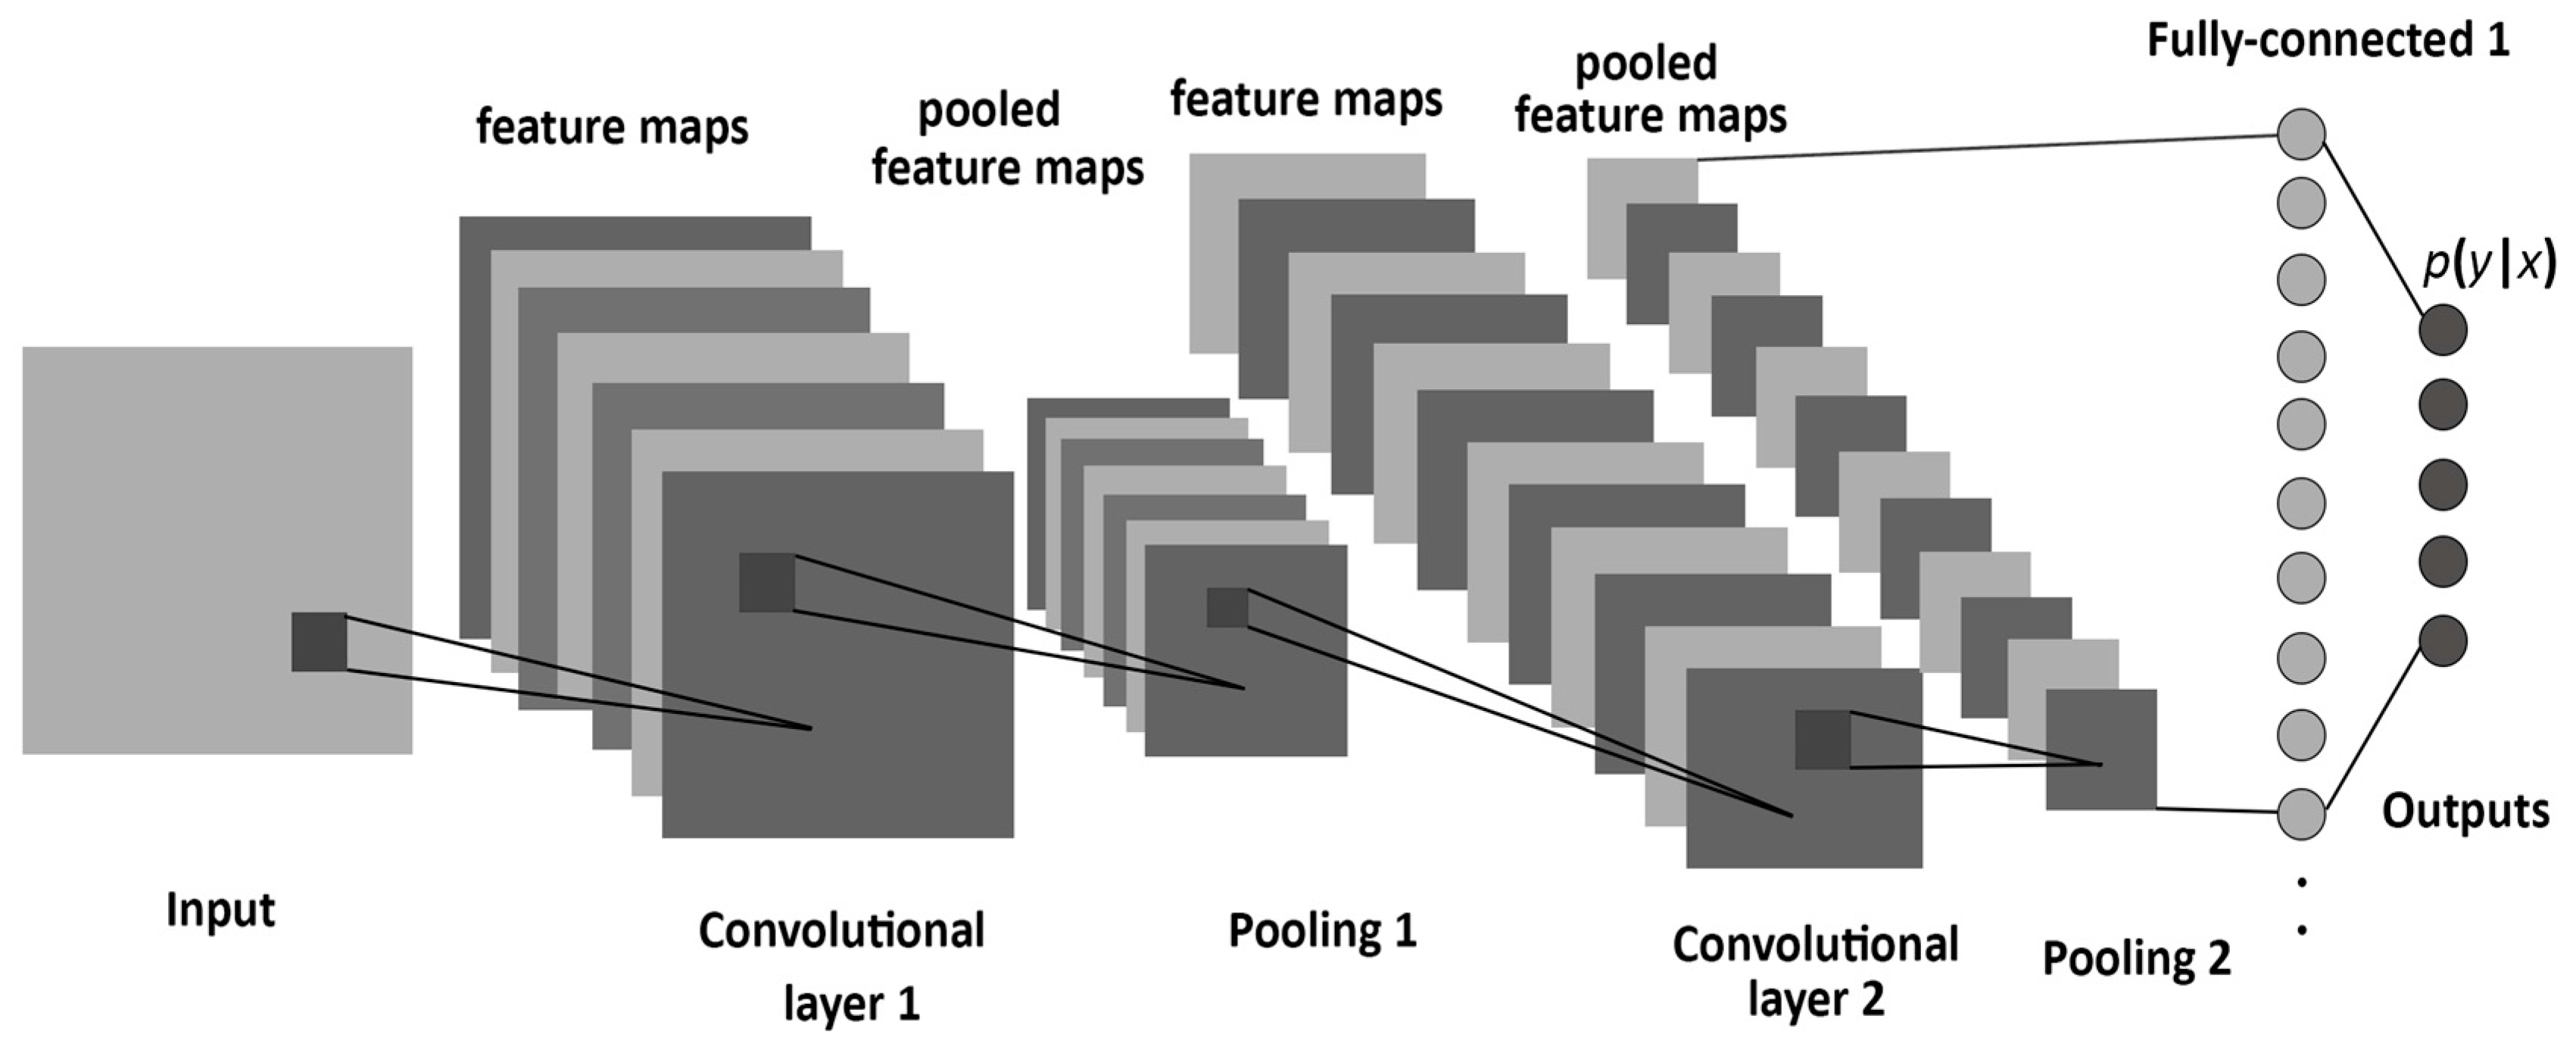
\includegraphics[width=1.0\textwidth]{../rc/images/cnn_architecture.png}
	\label{fig:cnn_architecture}
}


CNNs have the advantage of being able to automatically identify relevant features in images. As such, they are used for computer vision, object detection as well as classification tasks. In the demonstration for this work, the CNN architecture is used to classify the image and extract the relevant features.


\subsection{Recurrent Neural Networks}
\subsection{Reinforcement Learning}


\section{Existing Approaches}

Raster to vector conversion is a well researched field, and there are many different approaches on how to do it. Apart from algorithm based strategies, machine learning and particularly neural networks are promising and in active development \cite{dziuba_image_2023}.

\subsection{Algorithmic Approaches}

\begin{enumerate}[label=\Roman*]
   \item \textbf{Edge Detection Techniques} Traditional algorithms often rely on edge detection methods to identify boundaries in raster images. These can be used to identify the shapes in the image, which can then be used to generate its vector representation.

   \item \textbf{Hough Transform} The Hough Transform is utilized to detect lines in raster images, serving as a foundation for vectorization. This approach is effective in representing straight lines but may face challenges with curves.

   \item \textbf{Skeletonization} Skeletonization algorithms aim to reduce shapes in raster images to their core structures, facilitating the extraction of vector representations.
\end{enumerate}

\subsection{Deep Learning Approaches}

\begin{enumerate}[label=\Roman*]
   \item \textbf{Convolutional Neural Networks (CNNs)} CNNs have been employed for raster-to-vector conversion by learning hierarchical features. They excel in capturing spatial relationships and are effective in handling complex patterns.

   \item \textbf{Autoencoders} Autoencoders, especially variational autoencoders (VAEs), have shown promise in capturing latent representations of raster images, which can be used for vectorization.

   \item \textbf{Generative Adversarial Networks (GANs)} GANs, known for generating realistic images, can be adapted to generate vector representations by training on paired raster-vector data.

   \item \textbf{Recurrent Neural Networks (RNNs)} RNNs, with their sequential learning capability, are suitable for tasks involving sequential data. They can be applied to capture patterns in raster images that than can be used for vectorization.

   \item \textbf{Attention Mechanisms} Models incorporating attention mechanisms, such as Transformer architectures, can focus on relevant parts of raster images during the vectorization process, improving accuracy.
\end{enumerate}

These approaches represent a spectrum of techniques, each with its strengths and limitations. Hybrid models that combine algorithmic and deep learning components have also emerged, aiming to leverage the benefits of both paradigms. As one of those, MarVel




\chapter{Goal and Hypothesis}

To train a machine learning model to vectorization of raster images, a substantial amount of data is needed. Ideal data would be pairs of raster and vector representations of the same image, which are difficult to obtain normally. Since the conversion of vector images to raster formats is far less difficult, it could be a valid approach to generate random vector images and them convert them into a raster format, to get those raster-vector pairs on which the model can be trained.


This work examines this approach in regard to the following questions:

\begin{enumerate}[label=\Roman*]
   \item Is it feasible to approach raster to vector graphics conversion with a neural network that is trained on randomly generated data?
   \begin{enumerate}
      \item Can those pairs of raster and vector representations be randomly generated?
      \item Are there models that can learn to convert raster images to vector representations when trained on the generated data?
   \end{enumerate}
   \item What strategies or measures have to be taken to make this feasible?
   \item What are the limitations and pitfalls of this approach?
\end{enumerate}


\chapter{Method}

\section{Overview}

The training and evaluation data for the model is generated 

\section{Language Choice}

Deep learning is a very resource intense task, and since the work was limited in time and resource usage, the language choice was taken in regards mainly to the expected development time and runtime performance of the language and their frameworks. And since the computational intensive parts are done within the deep learning library that is going to be used, the availability of performant and established machine learning libraries was a high priority. On this basis, the table \ref{table:language_evaluation} has been produced, which assigns points to each of the important factors. 

\begin{table}
   \begin{tabular} {|c||p{2.2cm}|p{2.2cm}|p{2.5cm}|p{2.2cm}|p{2.2cm}|}
      \hline
      Language    & Performance & DL libraries & Names & Other libraries* & Other remarks \\
      \hline\hline
      Python      & 1 & 4 & 5 & Pytorch, TF & Gradually optimizable** \\ \hline
      Javascript  & 1 & 4 & 4 & BrainJS, Ml5 & Runs in the web \\ \hline
      C++         & 5 & 2 &   & TF &\\ \hline
      Rust        & 5 & 3 &   & Burn, Tangram &\\ \hline
      C           & 5 & 1 &   & Darknet &\\ \hline
      Go          & 5 & 2 &   & Gorgonia &\\
      \hline
   \end{tabular}
   \caption{Language evaluation table}
   \label{table:language_evaluation}
\end{table}

\subsection*{Python}
\begin{description}
   \item[Ecosystem] Many well established and highly optimized libraries such as TF, Keras, Pytorch.
   \item[Performance] Slow, but libraries are written mostly in C and heavily optimized. Performance critical parts can gradually be optimized by switching to Cyphon, a compiler which can take advantage of type information and call back and forth into Python and C.
\end{description}

\subsection*{Javascript}
\begin{description}
   \item[Ecosystem] Many high-level machine learning libraries such as Brain.js, Ml5.js but few allow the fine-grained control needed for deep learning research.
\end{description}


\subsection*{C++} High runtime performance, but low development speed. Attention in needed to keep it memory safe.
\begin{description}
   \item[Rust] High runtime performance and memory safe by default. Relies heavily on high level constructs which speeds up development 
   \item[C] Lack of high level features can slow down development speed. Not memory safe.
   \item[Go] Fast iterations. Deep learning ecosystem not yet mature.
\end{description}


\section{Framework Choice}
\section{Model Architecture}

The ability to automatically learn how to classify but also extract important features from images is what makes the CNN architecture suitable for this project. Consequentally, the model used in the demonstration sends the input image through two stacks of convolution layers with ReLU activation and Max Pooling layers.


\section{Data Generation}

The data that the model uses for training consists of raster images, with one shape in each of them. The images are internally represented as numpy arrays, where each entry represents the color values of a pixel. The background is white (i. e. RGB values set to (1, 1, 1)), and the pixels that fall within the shape are set to (0, 0, 0), thus appearing black, so that the contrast between shape and background is maximized.

All data generation is implemented in \lstinline{rtov/data/} and its subdirectories. A class, \lstinline{LazyDataset}, which inherits from the \lstinline{torch.utils.data.Dataset}, provides an interface, which a \lstinline{torch.utils.data.Dataloader} object can use later to get the next image. Therefore, the method \lstinline{__getitem__(self, i: int)} is provided, which loads a numpy array, draws a random shape on it and transforms it into a vector.

\section{Model Architecture}

The model in the demonstration is a convolutional neural network. It does

\section{Optimizing Mechanisms}

\subsection{Memory Management Pitfall}

Interesting is that the memory that holds the numpy array which represents the pixel values could be reused, which would have the to have the result that garbage collection is less often invoked. Since garbage collection can be a performance bottleneck      % TODO: Citation needed
, this can in some situation lead to significant performance improvements.      % TODO: Citation needed

Such a reusing of memory was tried to be achieved by using following code: \lstinline{self.image[:] = np.full(shape, ..)}. Manual memory management is usually not possible in Python, since it does not officially support it. Objects like arrays are usually passed by pointer, and by reassigning to a variable, this pointer is overwritten, leaving the old value in memory until the next garbage collection is invoked. Then the garbage collector frees the memory after finding out that no references to it exist anymore.      % TODO: Citation needed

In the case of numpy arrays though, \lstinline{[:]} can be used to explicitly dereference the numpy array.

\begin{lstlisting}
   import numpy as np
   a = np.array([[1, 2, 3], [4, 5, 6]])
   b = a       # Makes a copy of the pointer, not the object
   c = a

   c = 0       # `c` is changed
   print(a)    # `a` is still the same -> new object was created

   b[:] = 0    # Change `b`
   print(a)    # `a` has changed as well -> the same memory was overwritten
\end{lstlisting}

So \lstinline{a[:] = x} in Python, where \lstinline{a} is a numpy array is the equivalent to do \lstinline{*b = x;} in C in terms of memory access.




\chapter{Results}
% TODO


\chapter{Discussion}

\section{Opportunities of Generated Training Data for Vectorization}

The demonstration has shown that a deep learning model can be trained on raster-vector representation pairs that are generated randomly, and the results that it produces resemble the original image. In that regard the demonstration has confirmed the initial hypothesis.

It has to be considered though that the data that is used for the training is very limited and not yet on a point where it could be used in real world applications. It consists of a small number of shapes, and the model extracts only data concerning position and size of the shapes. It lacks the ability to determine the color of a shape, and cannot be used to convert images containing more than one shape and therefore the ability to recognize relations between the shapes in an image. The model outputs a numerical representation of the image, which first would have to be converted into the actual format. This should not be a problem though, since 
Those are limitations of demonstration and not necessarily of the approach itself. The model used in the demonstration cannot answer the question of whether those obstacles can be overcome or not.

Those observations could be made though:

\begin{enumerate}[label=\Roman*]
   \item Even a model trained on a CPU can quickly learn to extract shapes from raster images using the generated data
   \item To scale and improve the model, many optimizations could still be taken in the sections model architecture, training data and training parameter optimization
   \item No obstacles have been observed when changing the models training data. There is no apparent reason why it should not be possible to make a model learn more complex data.
   \item A more complex model may be needed for further experiments
\end{enumerate}


\section{Limitations}

\section{Proposed Model Architectures}

To be able to convert raster images to vector images using deep learning, there are many different strategies and architectures. In regard to the experience that was accumulated in the progress of this work, the following architecture is proposed for projects going further than this thesis does. It is a broad structure that includes elements of many different deep learning strategies such as Reinforcement learning, Recurrent convolutional networks using features from residual neural networks.

\begin{enumerate}
   \item The input is a raster image
   \item First layers are convolution-pooling layers, which are applied to the input image to extract features
   \item The output of layers just after or in the convolutional layers is passed directly to one or more small, independent fully connected layers. These layers are used to classify color and shape
   \item Second layers are fully connected layers, which are used to classify the features
   \item The output is then passed to another set of fully connected layers, which are specific for the shape that has already been predicted. These layers are used to extract the shape-specific data, such as position, rotation and corner points or size
   \item The output is then converted into a raster format, which then is compared to the input image, and the loss is a function of the difference between the two images

   \item Recurrent capabilities can be added, or the predicted shape can be removed from the image, such that the model can be called again to predict the next shape
\end{enumerate}

\section{Future Work}

\section{Conclusion}


\chapter{Sources and References}

\printbibliography



\end{document}
